\documentclass[tikz,border=10pt]{standalone}
\usetikzlibrary{shapes}
\usetikzlibrary{arrows}
\usetikzlibrary{positioning}
\begin{document} 

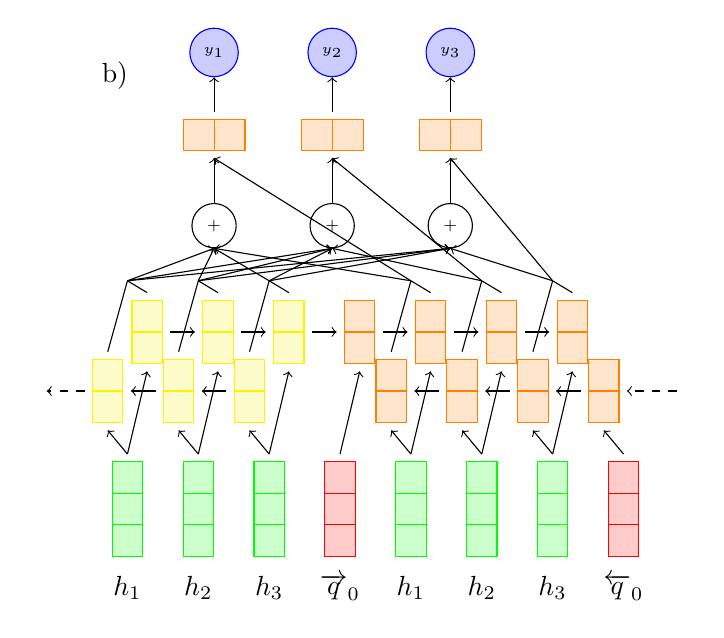
\begin{tikzpicture}[
  hid/.style 2 args={
    rectangle split,
    draw=#2,
    rectangle split parts=#1,
    fill=#2!20,
    outer sep=1mm},
  mlp/.style 2 args={
    rectangle split,
    rectangle split horizontal,
    draw=#2,
    rectangle split parts=#1,
    fill=#2!20,
    outer sep=1mm}
]

  \node [anchor=west] (label) at (.45, 4.5) {b)};

  \foreach \i [count=\step from 1] in {$h_1$, $h_2$, $h_3$} {
    \node (i\step) at (.9*\step, -2) {\i};
    \node[hid={3}{green}] (e\step) at (.9*\step, -1) {};    
  }
  \node (i4) at (.9*4, -2) {$\overrightarrow{q}_0$};
  \node[hid={3}{red}] (e4) at (.9*4, -1) {};    
  \foreach \i [count=\step from 5] in {$h_1$, $h_2$, $h_3$} {
    \node (i\step) at (.9*\step, -2) {\i};
    \node[hid={3}{green}] (e\step) at (.9*\step, -1) {};    
  }
  \node (i8) at (.9*8, -2) {$\overleftarrow{q}_0$};
  \node[hid={3}{red}] (e8) at (.9*8, -1) {};    

  \foreach \step in {1,...,3} {
    \node[hid={2}{yellow}] (h_r_\step) at (-.25 + .9 *\step, .5) {};    
    \node[hid={2}{yellow}] (h_f_\step) at (.25 + .9 *\step, 1.25) {};    
    \draw[->] (e\step.north) -> (h_f_\step.south);
    \draw[->] (e\step.north) -> (h_r_\step.south);
%    \node[mlp={2}{yellow}] (h_\step) at (.9 *\step, 2.5) {};    
%    \node[circle, draw=blue, fill=blue!20] (y_\step) at (.9 *\step, 3.75) {$y_\step$};    
%    \draw[->] (h_\step.north) -> (y_\step.south);
%    \draw[->] (h_f_\step.north) -> (h_\step.south);
%    \draw[->] (h_r_\step.north) -> (h_\step.south);
  }

  \foreach \step in {5,...,8} {
    \node[hid={2}{orange}] (h_r_\step) at (-.25 + .9 *\step, .5) {};    
    \draw[->] (e\step.north) -> (h_r_\step.south);
  }
  \foreach \step in {4,...,7} {
    \node[hid={2}{orange}] (h_f_\step) at (.25 + .9 *\step, 1.25) {};    
    \draw[->] (e\step.north) -> (h_f_\step.south);
%    \draw[->] (e\step.north) -> (h_r_\step.south);
%    \node[mlp={2}{yellow}] (h_\step) at (.9 *\step, 2.5) {};    
%    \node[circle, draw=blue, fill=blue!20] (y_\step) at (.9 *\step, 3.75) {$y_\step$};    
%    \draw[->] (h_\step.north) -> (y_\step.south);
%    \draw[->] (h_f_\step.north) -> (h_\step.south);
%    \draw[->] (h_r_\step.north) -> (h_\step.south);

  }

  \draw[->] (h_f_1.east) -> (h_f_2.west);
  \draw[->] (h_f_2.east) -> (h_f_3.west);
  \draw[->] (h_f_3.east) -> (h_f_4.west);
  \draw[->] (h_f_4.east) -> (h_f_5.west);
  \draw[->] (h_f_5.east) -> (h_f_6.west);
  \draw[->] (h_f_6.east) -> (h_f_7.west);
 
  \draw[->] (h_r_3.west) -> (h_r_2.east);
  \draw[->] (h_r_2.west) -> (h_r_1.east);
  \node (lborder) at (-.25 + .9 * 0, .5) {};
  \node (rborder) at (-.1 + .9 * 9, .5) {};
  \draw[->,dashed] (h_r_1.west) -- (lborder);
  \draw[->,dashed] (rborder) -- (h_r_8.east);
  \draw[->] (h_r_8.west) -> (h_r_7.east);
  \draw[->] (h_r_7.west) -> (h_r_6.east);
  \draw[->] (h_r_6.west) -> (h_r_5.east);

  \node[circle,draw=black] (attn1) at (2, 2.6) {\tiny$+$};    
  \node[circle,draw=black] (attn2) at (3.5, 2.6) {\tiny$+$};    
  \node[circle,draw=black] (attn3) at (5, 2.6) {\tiny$+$};    
  
  \node[mlp={2}{orange}] (h1) at (2, 3.75) {};
  \node[mlp={2}{orange}] (h2) at (3.5, 3.75) {};
  \node[mlp={2}{orange}] (h3) at (5, 3.75) {};
  \node[circle, draw=blue, fill=blue!20] (y1) at (2, 4.8) {\tiny $y_1$};    
  \node[circle, draw=blue, fill=blue!20] (y2) at (3.5, 4.8) {\tiny $y_2$};    
  \node[circle, draw=blue, fill=blue!20] (y3) at (5, 4.8) {\tiny $y_3$};    

  \foreach \step in {1,...,3} {
      \node (m\step) at (\step * .9, 1.9) {};
      \path[draw=black,-] (h_f_\step.north) -- (m\step.center);
      \path[draw=black,-] (h_r_\step.north) -- (m\step.center);
      \foreach \stepj in {1,...,3} {
          \path[draw=black,->] (m\step.center) -- (attn\stepj.south);
      } 
  }

  \foreach \step in {1,...,3} {
      \path[draw=black,->] (attn\step.north) -- (h\step.south);
      \path[draw=black,->] (h\step.north) -- (y\step.south);
  }


  \node (m21) at (5* .9, 1.9) {};
  \path[draw=black,-] (h_f_5.north) -- (m21.center);
  \path[draw=black,-] (h_r_5.north) -- (m21.center);
  \path[draw=black,->] (m21.center) -- (attn1.south);
  \path[draw=black,->] (m21.center) -- (h1.south);

  \node (m22) at (6* .9, 1.9) {};
  \path[draw=black,-] (h_f_6.north) -- (m22.center);
  \path[draw=black,-] (h_r_6.north) -- (m22.center);
  \path[draw=black,->] (m22.center) -- (attn2.south);
  \path[draw=black,->] (m22.center) -- (h2.south);


  \node (m23) at (7* .9, 1.9) {};
  \path[draw=black,-] (h_f_7.north) -- (m23.center);
  \path[draw=black,-] (h_r_7.north) -- (m23.center);
  \path[draw=black,->] (m23.center) -- (attn3.south);
  \path[draw=black,->] (m23.center) -- (h3.south);




\end{tikzpicture}


\end{document}
